\PassOptionsToPackage{unicode=true}{hyperref} % options for packages loaded elsewhere
\PassOptionsToPackage{hyphens}{url}
%
\documentclass[11pt,ignorenonframetext,]{beamer}
\usepackage{pgfpages}
\setbeamertemplate{caption}[numbered]
\setbeamertemplate{caption label separator}{: }
\setbeamercolor{caption name}{fg=normal text.fg}
\beamertemplatenavigationsymbolsempty
% Prevent slide breaks in the middle of a paragraph:
\widowpenalties 1 10000
\raggedbottom
\setbeamertemplate{part page}{
\centering
\begin{beamercolorbox}[sep=16pt,center]{part title}
  \usebeamerfont{part title}\insertpart\par
\end{beamercolorbox}
}
\setbeamertemplate{section page}{
\centering
\begin{beamercolorbox}[sep=12pt,center]{part title}
  \usebeamerfont{section title}\insertsection\par
\end{beamercolorbox}
}
\setbeamertemplate{subsection page}{
\centering
\begin{beamercolorbox}[sep=8pt,center]{part title}
  \usebeamerfont{subsection title}\insertsubsection\par
\end{beamercolorbox}
}
\AtBeginPart{
  \frame{\partpage}
}
\AtBeginSection{
  \ifbibliography
  \else
    \frame{\sectionpage}
  \fi
}
\AtBeginSubsection{
  \frame{\subsectionpage}
}
\usepackage{lmodern}
\usepackage{amssymb,amsmath}
\usepackage{ifxetex,ifluatex}
\usepackage{fixltx2e} % provides \textsubscript
\ifnum 0\ifxetex 1\fi\ifluatex 1\fi=0 % if pdftex
  \usepackage[T1]{fontenc}
  \usepackage[utf8]{inputenc}
  \usepackage{textcomp} % provides euro and other symbols
\else % if luatex or xelatex
  \usepackage{unicode-math}
  \defaultfontfeatures{Ligatures=TeX,Scale=MatchLowercase}
\fi
\usetheme[]{Montpellier}
\usecolortheme{beaver}
% use upquote if available, for straight quotes in verbatim environments
\IfFileExists{upquote.sty}{\usepackage{upquote}}{}
% use microtype if available
\IfFileExists{microtype.sty}{%
\usepackage[]{microtype}
\UseMicrotypeSet[protrusion]{basicmath} % disable protrusion for tt fonts
}{}
\IfFileExists{parskip.sty}{%
\usepackage{parskip}
}{% else
\setlength{\parindent}{0pt}
\setlength{\parskip}{6pt plus 2pt minus 1pt}
}
\usepackage{hyperref}
\hypersetup{
            pdftitle={Etude des effets des pésticides dans la production des vins de table},
            pdfauthor={A. Blanc, N. Gusarov, S. Picon},
            pdfborder={0 0 0},
            breaklinks=true}
\urlstyle{same}  % don't use monospace font for urls
\newif\ifbibliography
\usepackage{graphicx,grffile}
\makeatletter
\def\maxwidth{\ifdim\Gin@nat@width>\linewidth\linewidth\else\Gin@nat@width\fi}
\def\maxheight{\ifdim\Gin@nat@height>\textheight\textheight\else\Gin@nat@height\fi}
\makeatother
% Scale images if necessary, so that they will not overflow the page
% margins by default, and it is still possible to overwrite the defaults
% using explicit options in \includegraphics[width, height, ...]{}
\setkeys{Gin}{width=\maxwidth,height=\maxheight,keepaspectratio}
\setlength{\emergencystretch}{3em}  % prevent overfull lines
\providecommand{\tightlist}{%
  \setlength{\itemsep}{0pt}\setlength{\parskip}{0pt}}
\setcounter{secnumdepth}{0}

% set default figure placement to htbp
\makeatletter
\def\fps@figure{htbp}
\makeatother

\usepackage{array}
\usepackage{multicol}

\title{Etude des effets des pésticides dans la production des vins de table}
\providecommand{\subtitle}[1]{}
\subtitle{Analyse empirique des marchés}
\author{A. Blanc, N. Gusarov, S. Picon}
\providecommand{\institute}[1]{}
\institute{Université Grenoble Alpes}
\date{11/12/2019}

\begin{document}
\frame{\titlepage}

\begin{frame}
\tableofcontents[hideallsubsections]
\end{frame}
\begin{frame}{Introduction}
\protect\hypertarget{introduction}{}

\end{frame}

\begin{frame}{Plan de la présentation}
\protect\hypertarget{plan-de-la-presentation}{}

\begin{itemize}
\tightlist
\item
  Présentation de la problématique
\item
  Présentation des données
\item
  Modélisation
\item
  Les résultats
\end{itemize}

\end{frame}

\begin{frame}{Le problème des pesticides}
\protect\hypertarget{le-probleme-des-pesticides}{}

\begin{itemize}
\tightlist
\item
  Présentation du problème des pésticides
\item
  Etat actuel
\item
  Comment combattre
\end{itemize}

\end{frame}

\begin{frame}{Le marché du vin français}
\protect\hypertarget{le-marche-du-vin-francais}{}

\begin{itemize}
\tightlist
\item
  Le marché commun
\item
  Utilisation des pésticides
\item
  Heterogénéité
\item
  Pourquoi vins de table
\end{itemize}

\end{frame}

\begin{frame}{Le Modèle théorique}
\protect\hypertarget{le-modele-theorique}{}

\begin{itemize}
\tightlist
\item
  Le rôle des pesticides dans la production du vin
\item
  Le rôle de la demande sur la production et l'offre en général
\item
  La formalisation et les équations
\end{itemize}

\end{frame}

\begin{frame}{Les données}
\protect\hypertarget{les-donnees}{}

\begin{itemize}
\tightlist
\item
  Dimentions :

  \begin{itemize}
  \tightlist
  \item
    Départements
  \item
    Années
  \end{itemize}
\item
  Les variables :

  \begin{itemize}
  \tightlist
  \item
    Pésticides (quantités)
  \item
    Vins (quantités produits, prix)
  \item
    Variables de controle (revenus, surface cultivé)
  \end{itemize}
\end{itemize}

\end{frame}

\begin{frame}{Les statistiques déscriptives}
\protect\hypertarget{les-statistiques-descriptives}{}

\begin{itemize}
\tightlist
\item
  Between and within variance par variable
\item
  Bivariate plots with support regressions
\item
  Covariance analysis
\item
  Fixed vs Random effects
\end{itemize}

\end{frame}

\begin{frame}{Etude de la variance}
\protect\hypertarget{etude-de-la-variance}{}

\tiny
\begin{table}[!htbp] \centering 
  \caption{Variance study}
\begin{tabular}{@{\extracolsep{5pt}} l|cccc} 
\\[-1.8ex]\hline 
\hline \\[-1.8ex] 
 & Mean & Overall & Between & Within \\ 
\hline \\[-1.8ex] 
Index prix & $0.175$ & $0.568$ & $0.368$ & $0.434$ \\ 
Index pesticides & $0.170$ & $0.333$ & $0.239$ & $0.234$ \\ 
Surface & $4.892$ & $1.986$ & $1.955$ & $0.410$ \\ 
Revenus & $9.891$ & $0.061$ & $0.061$ & $0.011$ \\ 
Temps & $3$ & $1.416$ & $0$ & $1.416$ \\ 
\hline \\[-1.8ex] 
\end{tabular} 
\end{table}

\end{frame}

\begin{frame}{Visualisatoin des interdependances}
\protect\hypertarget{visualisatoin-des-interdependances}{}

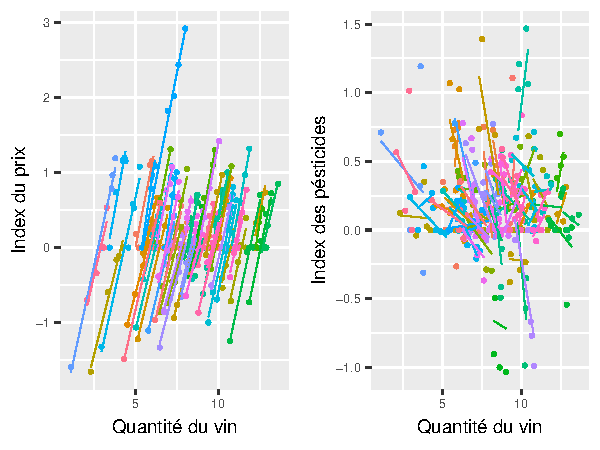
\includegraphics{Presentation_files/figure-beamer/unnamed-chunk-12-1.pdf}

\end{frame}

\begin{frame}{Visualisatoin des interdependances}
\protect\hypertarget{visualisatoin-des-interdependances-1}{}

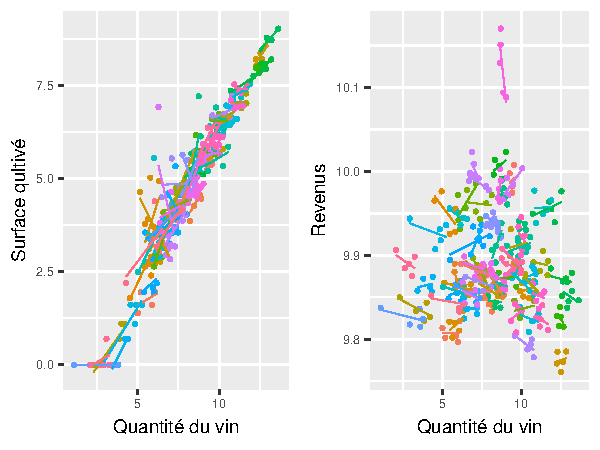
\includegraphics{Presentation_files/figure-beamer/unnamed-chunk-13-1.pdf}

\end{frame}

\begin{frame}{Random and fixed effects testing}
\protect\hypertarget{random-and-fixed-effects-testing}{}

\begin{itemize}
\tightlist
\item
  Poolability tests (tested versus pooled model)
\end{itemize}

\tiny
\begin{table}[!htbp] \centering
  \caption{Chow pooling test, p-values}
\begin{tabular}{@{\extracolsep{5pt}} l|cc} 
\\[-1.8ex]\hline 
\hline \\[-1.8ex] 
 & Random & Fixed \\ 
\hline \\[-1.8ex] 
Index prix & $0.535$ & $0.533$ \\ 
Index pesticides & $0.485$ & $0.451$ \\ 
Surface & $0$ & $0.0001$ \\ 
Revenus & $0.297$ & $0.247$ \\ 
\hline \\[-1.8ex]
\end{tabular} 
\end{table}

\end{frame}

\begin{frame}{Type of fixed effect testing}
\protect\hypertarget{type-of-fixed-effect-testing}{}

\begin{itemize}
\tightlist
\item
  Type of fixed effects testing
\end{itemize}

\tiny
\begin{table}[!htbp] \centering 
  \caption{Lagrange multiplier test, p-values}
\begin{tabular}{@{\extracolsep{5pt}} l|ccc} 
\\[-1.8ex]\hline 
\hline \\[-1.8ex] 
 & Individual & Time & Two-ways \\ 
\hline \\[-1.8ex] 
Index prix & $0$ & $0.169$ & $0$ \\ 
Index pesticides & $0$ & $0.222$ & $0$ \\ 
Surface & $0$ & $0.030$ & $0$ \\ 
Revenus & $0$ & $0.248$ & $0$ \\ 
\hline \\[-1.8ex] 
\end{tabular} 
\end{table}

\end{frame}

\begin{frame}{Correlation}
\protect\hypertarget{correlation}{}

\tiny
\begin{table}[!htbp] \centering
  \tiny\caption{Overall correlation}
\begin{tabular}{@{\extracolsep{5pt}} l|cccccc}
\\[-1.8ex]\hline
\hline \\[-1.8ex]
 & Quantité du vin & IP & Surface & Revenus & Index pésticides & Temps \\
\hline \\[-1.8ex]
Quantité du vin & $1$ & $0.154$ & $0.956$ & $-0.027$ & $-0.078$ & $-0.036$ \\      
IP & $0.154$ & $1$ & $0.045$ & $-0.037$ & $-0.127$ & $0.043$ \\
Surface & $0.956$ & $0.045$ & $1$ & $-0.057$ & $-0.060$ & $-0.064$ \\
Revenus & $-0.027$ & $-0.037$ & $-0.057$ & $1$ & $-0.052$ & $0.119$ \\
Index pésticides & $-0.078$ & $-0.127$ & $-0.060$ & $-0.052$ & $1$ & $0.291$ \\  
Temps & $-0.036$ & $0.043$ & $-0.064$ & $0.119$ & $0.291$ & $1$ \\
\hline \\[-1.8ex]
\end{tabular}
\end{table}

\tiny
\begin{table}[!htbp] \centering 
  \tiny\caption{Within transformation correlation}
\begin{tabular}{@{\extracolsep{5pt}} ccccccc} 
\\[-1.8ex]\hline 
\hline \\[-1.8ex] 
 & Quantité du vin & IP & Surface & Revenus & Index pésticides & Temps \\ 
\hline \\[-1.8ex] 
Quantité du vin & $1$ & $0.961$ & $0.366$ & $-0.160$ & $-0.228$ & $-0.199$ \\ 
IP & $0.961$ & $1$ & $0.289$ & $-0.009$ & $-0.127$ & $0.056$ \\ 
Surface & $0.366$ & $0.289$ & $1$ & $-0.166$ & $-0.191$ & $-0.310$ \\ 
Revenus & $-0.160$ & $-0.009$ & $-0.166$ & $1$ & $0.228$ & $0.652$ \\ 
Index pésticides & $-0.228$ & $-0.127$ & $-0.191$ & $0.228$ & $1$ & $0.414$ \\ 
Temps & $-0.199$ & $0.056$ & $-0.310$ & $0.652$ & $0.414$ & $1$ \\ 
\hline \\[-1.8ex] 
\end{tabular} 
\end{table}

\end{frame}

\begin{frame}{Within transformation results}
\protect\hypertarget{within-transformation-results}{}

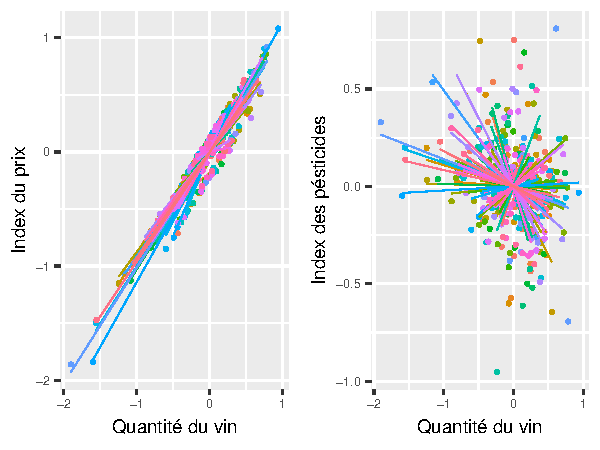
\includegraphics{Presentation_files/figure-beamer/unnamed-chunk-22-1.pdf}

\end{frame}

\begin{frame}{Within transformation results}
\protect\hypertarget{within-transformation-results-1}{}

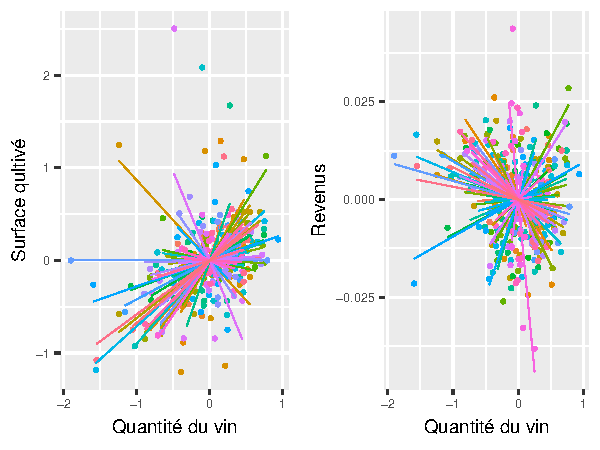
\includegraphics{Presentation_files/figure-beamer/unnamed-chunk-23-1.pdf}

\end{frame}

\begin{frame}{Modèlisation}
\protect\hypertarget{modelisation}{}

\begin{itemize}
\tightlist
\item
  Explication de la méthode utilisée

  \begin{itemize}
  \tightlist
  \item
    Panel data

    \begin{itemize}
    \tightlist
    \item
      Within transforation
    \item
      Fixed effects
    \item
      Obtained slopes are averages for all population
    \end{itemize}
  \item
    AIDS model

    \begin{itemize}
    \tightlist
    \item
      Interdependent equations (simultaneity bias)
    \item
      3SLS estimator (that is identical to ILS estimator)
    \item
      It generates consistent estimates
    \item
      The distribution of the estimators are normally distributed only
      in large samples
    \item
      The estimator is (asymptotically) efficient
    \end{itemize}
  \end{itemize}
\item
  Limites du modèle

  \begin{itemize}
  \tightlist
  \item
    Faible representation des effets hetérogenes entre les régions (nous
    estimons seulemnt les effets moyens)
  \item
    Les interferences induites par l'heterogénéité
  \end{itemize}
\end{itemize}

\end{frame}

\begin{frame}{Résultats d'estimation}
\protect\hypertarget{resultats-destimation}{}

\begin{itemize}
\tightlist
\item
  Les coefficients estimés avec leurs variance
\item
  Etude des erreurs
\item
  Vérification des hypothèses (5 hypothèses) :

  \begin{itemize}
  \tightlist
  \item
    La moyenne nulle des erreurs
  \item
    Homoscedacité
  \item
    Autocorrélation
  \item
    Spécification du modèle
  \item
    \ldots{} (à voir)
  \end{itemize}
\end{itemize}

\end{frame}

\begin{frame}{Les résultats OLS vs SUR}
\protect\hypertarget{les-resultats-ols-vs-sur}{}

\tiny

\begin{table}
\begin{center}
\begin{tabular}{l c c c }
\hline
 & OLS & WLS & SUR \\
\hline
Demande: ipi        & $0.93^{***}$  & $0.93^{***}$  & $0.93^{***}$  \\
                    & $(0.01)$      & $(0.01)$      & $(0.01)$      \\
Demande: ri         & $-5.75^{***}$ & $-5.75^{***}$ & $-2.00^{***}$ \\
                    & $(0.47)$      & $(0.47)$      & $(0.33)$      \\
Offre: ipi          & $0.90^{***}$  & $0.90^{***}$  & $0.92^{***}$  \\
                    & $(0.01)$      & $(0.01)$      & $(0.01)$      \\
Offre: si           & $0.08^{***}$  & $0.08^{***}$  & $0.02^{*}$    \\
                    & $(0.01)$      & $(0.01)$      & $(0.01)$      \\
Offre: iki          & $-0.17^{***}$ & $-0.17^{***}$ & $-0.05^{**}$  \\
                    & $(0.02)$      & $(0.02)$      & $(0.02)$      \\
\hline
Demande: R$^2$      & 0.95          & 0.95          & 0.94          \\
Offre: R$^2$        & 0.94          & 0.94          & 0.93          \\
Demande: Adj. R$^2$ & 0.95          & 0.95          & 0.94          \\
Offre: Adj. R$^2$   & 0.94          & 0.94          & 0.93          \\
Num. obs. (total)   & 690           & 690           & 690           \\
\hline
\multicolumn{4}{l}{\scriptsize{$^{***}p<0.001$, $^{**}p<0.01$, $^*p<0.05$}}
\end{tabular}
\caption{Statistical models}
\label{table : ols, wls and sur}
\end{center}
\end{table}
\tiny

\end{frame}

\begin{frame}{Disturbances correlation study}
\protect\hypertarget{disturbances-correlation-study}{}

\begin{itemize}
\tightlist
\item
  Les résidus sont non correlés avec les variables explicatives
\end{itemize}

\tiny
\begin{table}[!htbp] \centering 
  \caption{Errors correlation}
\begin{tabular}{@{\extracolsep{5pt}} cccccccc} 
\\[-1.8ex]\hline 
\hline \\[-1.8ex] 
 & Vin & IP & Surface & Revenus & Pesticides & Demande & Offre \\ 
\hline \\[-1.8ex] 
Vin & $1$ & $0.961$ & $0.366$ & $-0.160$ & $-0.228$ & $0.232$ & $0.244$ \\ 
IP & $0.961$ & $1$ & $0.289$ & $-0.009$ & $-0.127$ & $-0$ & $-0$ \\ 
Surface & $0.366$ & $0.289$ & $1$ & $-0.166$ & $-0.191$ & $0.271$ & $-0$ \\ 
Revenus & $-0.160$ & $-0.009$ & $-0.166$ & $1$ & $0.228$ & $0$ & $-0.480$ \\ 
Pesticides & $-0.228$ & $-0.127$ & $-0.191$ & $0.228$ & $1$ & $-0.308$ & $-0$ \\ 
Demande & $0.232$ & $-0$ & $0.271$ & $0$ & $-0.308$ & $1$ & $0.740$ \\ 
Offre & $0.244$ & $-0$ & $-0$ & $-0.480$ & $-0$ & $0.740$ & $1$ \\ 
\hline \\[-1.8ex] 
\end{tabular} 
\end{table}

\end{frame}

\begin{frame}{Les résultats 2SLS, W2SLS et 3SLS}
\protect\hypertarget{les-resultats-2sls-w2sls-et-3sls}{}

\tiny

\begin{table}
\begin{center}
\begin{tabular}{l c c c }
\hline
 & 2SLS & W2SLS & 3SLS \\
\hline
Demande: ipi        & $1.19^{***}$  & $1.19^{***}$  & $1.19^{***}$  \\
                    & $(0.06)$      & $(0.06)$      & $(0.06)$      \\
Demande: ri         & $-5.67^{***}$ & $-5.67^{***}$ & $-5.67^{***}$ \\
                    & $(0.71)$      & $(0.71)$      & $(0.71)$      \\
Offre: ipi          & $-1.22$       & $-1.22$       & $-0.71$       \\
                    & $(1.97)$      & $(1.97)$      & $(1.96)$      \\
Offre: si           & $0.70$        & $0.70$        & $0.46$        \\
                    & $(0.59)$      & $(0.59)$      & $(0.58)$      \\
Offre: iki          & $-0.46$       & $-0.46$       & $-0.73^{*}$   \\
                    & $(0.34)$      & $(0.34)$      & $(0.32)$      \\
\hline
Demande: R$^2$      & 0.88          & 0.88          & 0.88          \\
Offre: R$^2$        & -3.37         & -3.37         & -1.60         \\
Demande: Adj. R$^2$ & 0.88          & 0.88          & 0.88          \\
Offre: Adj. R$^2$   & -3.40         & -3.40         & -1.62         \\
Num. obs. (total)   & 690           & 690           & 690           \\
\hline
\multicolumn{4}{l}{\scriptsize{$^{***}p<0.001$, $^{**}p<0.01$, $^*p<0.05$}}
\end{tabular}
\caption{Statistical models}
\label{table : 2sls, w2sls and 3sls}
\end{center}
\end{table}
\tiny

\end{frame}

\begin{frame}{Model choice tests}
\protect\hypertarget{model-choice-tests}{}

\begin{itemize}
\item
  Hausman 3SLS consistency test :

  Hausman specification test for consistency of the 3SLS estimation
\end{itemize}

data: dataWX Hausman = 5.5763, df = 5, p-value = 0.3497

\begin{itemize}
\tightlist
\item
  Likelihood test :
\end{itemize}

\tiny
\begin{table}[!htbp] \centering 
\begin{tabular}{@{\extracolsep{5pt}} cccccc} 
\\[-1.8ex]\hline 
\hline \\[-1.8ex] 
 & \#Df & LogLik & Df & Chisq & Pr(\textgreater Chisq) \\ 
\hline \\[-1.8ex] 
2SLS & $6$ & $152.708$ & $$ & $$ & $$ \\ 
3SLS & $7$ & $-149.621$ & $1$ & $604.657$ & $0$ \\ 
\hline \\[-1.8ex] 
\end{tabular} 
\end{table}

\end{frame}

\begin{frame}{Residuals tests for 3SLS}
\protect\hypertarget{residuals-tests-for-3sls}{}

\begin{itemize}
\tightlist
\item
  Residuals normality test (Shapiro-Wilk)

  \begin{itemize}
  \item
    Equation de la demande : {[}1{]} 2.882578e-05
  \item
    Equation de l'offre : {[}1{]} 2.976186e-07
  \end{itemize}
\item
  Residuals heteroscedasticity test (Bartlett test)

  \begin{itemize}
  \item
    Equation de la demande : {[}1{]} 0.9752152
  \item
    Equation de l'offre : {[}1{]} 0.00197632
  \end{itemize}
\end{itemize}

\end{frame}

\begin{frame}{Residuals autocorrelation study}
\protect\hypertarget{residuals-autocorrelation-study}{}

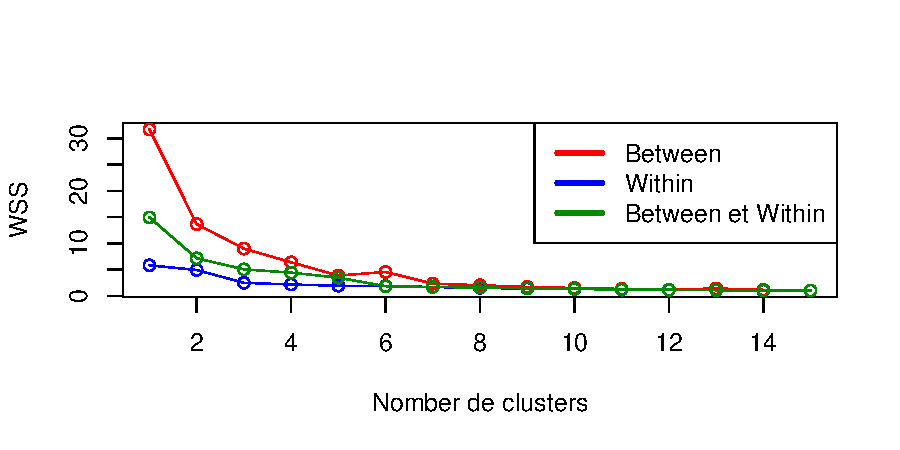
\includegraphics{Presentation_files/figure-beamer/unnamed-chunk-41-1.pdf}

\end{frame}

\begin{frame}{Disturbances correlation study for 2SLS}
\protect\hypertarget{disturbances-correlation-study-for-2sls}{}

\begin{itemize}
\tightlist
\item
  Les résidus sont peux correlés avec les variables explicatives
\end{itemize}

\tiny
\begin{table}[!htbp] \centering 
  \caption{Errors correlation}
\begin{tabular}{@{\extracolsep{5pt}} cccccccc} 
\\[-1.8ex]\hline 
\hline \\[-1.8ex] 
 & Vin & IP & Surface & Revenus & Pesticides & Demande & Offre \\ 
\hline \\[-1.8ex] 
Vin & $1$ & $0.961$ & $0.366$ & $-0.160$ & $-0.228$ & $-0.561$ & $0.898$ \\
IP & $0.961$ & $1$ & $0.289$ & $-0.009$ & $-0.127$ & $-0.746$ & $0.938$ \\
Surface & $0.366$ & $0.289$ & $1$ & $-0.166$ & $-0.191$ & $-0.034$ & $0.032$ \\ 
Revenus & $-0.160$ & $-0.009$ & $-0.166$ & $1$ & $0.228$ & $-0$ & $0$ \\
Pesticides & $-0.228$ & $-0.127$ & $-0.191$ & $0.228$ & $1$ & $-0.113$ & $0.105$ \\ 
Demande & $-0.561$ & $-0.746$ & $-0.034$ & $-0$ & $-0.113$ & $1$ & $-0.705$ \\ 
Offre & $0.898$ & $0.938$ & $0.032$ & $0$ & $0.105$ & $-0.705$ & $1$ \\ 
\hline \\[-1.8ex] 
\end{tabular} 
\end{table}

\end{frame}

\begin{frame}{Conclusions}
\protect\hypertarget{conclusions}{}

\begin{itemize}
\tightlist
\item
  Le rôle des pésticides
\item
  Le marché du vin
\item
  Validité
\item
  Limitations
\item
  Ouverture
\end{itemize}

\end{frame}

\begin{frame}{Bibliographie}
\protect\hypertarget{bibliographie}{}

\begin{itemize}
\tightlist
\item
  Inclure seulement les articles importants
\item
  Faire des réferences et mentionner ces articles dans la partie
  théorique
\end{itemize}

\end{frame}

\end{document}
